\chapter{Cellular Communication Technology}
\label{chpt:celltech}
\section{Introduction}
 Wireless technology is used by modern electronic devices to establish communication over which information is exchanged\cite{Karen2004}. Wireless technology facilitates communication between two devices by transmitting data or voice via a radio frequency\cite{Karen2004}. Examples of devices exchanging information wirelessly are radios for audio entertainment; television remotes to change frequencies; cellular phones for communication; wireless access points to create wireless LANs\cite{Karen2004}.

The popularity and rapid adoption of wireless technology contributes to the difficulty of planning, managing and operating wireless networks\cite{Karen2004}. As the popularity and use of services that use wireless technology increase, the need for these services to use different radio frequencies to communicate becomes greater\cite{wirelesstelcoMullet}. This need arises due to an effect called \emph{interference}, which occurs when two or more connections between devices use the same radio frequency to facilitate communication\cite{wirelesstelcoMullet}. This effect is discussed in more detail in chapter 3.

A wireless cellular operator is not allowed to operate on just any frequency. A governing body licenses a certain piece of the available wireless spectrum to the operator for use in their network\cite{FAPRAMColouring}. These frequencies that need to be licensed for use are known as \emph{commercial} frequencies and are very scarce as it is immensely expensive to license\cite{FAPRAMColouring}. 

The use of frequencies by services must be carefully considered to avoid interference when devices communicate with each other. This is a problem as the amount of devices that communicate far outstrips the amount of frequencies available for communication\cite{wirelesstelcoMullet}. Thus assigning frequencies to devices for communication is a difficult problem and is referred to as the \gls{FAP}\cite{Karen2004,Eisenblatter}.

Initially manual techniques were used to assign frequencies in an attempt to solve the \gls{FAP}\cite{Karen2004}. As a result, assigning frequencies was either too complex or just too daunting because of the sheer number of devices that needed to be assigned frequencies\cite{Karen2004}. Also, because of the rapid adoption of wireless technology the assignment of frequencies needed to be dynamic and hence automated\cite{Karen2004}.

By understanding how a \gls{gsm} network operates, especially how communication is facilitated, the reader is able to understand the problem this dissertation addresses. Therefore, this chapter will start off with section~\ref{sec:GSMNet} within which a brief history of \gls{gsm} networks are presented. Section~\ref{sec:GSMArch} follows the history discussion and presents an overview on the different architectural components the form a \gls{gsm} network. In section~\ref{sec:gsminterfaces} the different interfaces used by \gls{gsm} network components for communication is presented. Section~\ref{sec:interfacech} presents an overview on the logical frequencies that frequencies get divided into when used in a \gls{gsm} network. Finally this chapter concludes with a discussion on the handover process in section~\ref{sec:handover}.

\section{GSM Networks}
\label{sec:GSMNet}
The \gls{gsm} is a system for multiservice cellular communication that is capable of providing voice as well as data services\cite{GSMArchitectureProtocolsServices,wirelesstelcoMullet}. Most cellular networks in operation are \gls{gsm} based\cite{Karen2004,wirelesstelcoMullet}. The primary service that \gls{gsm} caters for is voice communication, but other data services such as \gls{SMS}, \gls{MMS} and internet connectivity services, e.g. \gls{GPRS}, \gls{EDGE} and \gls{HSCSD}, are becoming more important\cite{GSMArchitectureProtocolsServices,Eisenblatter}.

\Gls{gsm} is one of the most widely used radio communication technologies, which is why one needs to look at the history behind it in order to understand the domain of radio communication better \cite{GSMArchitectureProtocolsServices}. A brief history of the \gls{gsm} network specification will now be presented in the next section.

\subsection{A Brief History of GSM Networks}
\label{sec:gsmhistory}
In early 1981 a group known as the \emph{Groupe Speciale Mobile} was established to develop a Europe-wide radio communication system using the reserved 900 MHz band\footnote{In 1990 the United Kingdom requested that 1800 MHz band be added to the scope of the Groupe Speciale Mobile standard group. This variant of the \gls{gsm} specification became known as the \gls{DCS1800} \cite{GSM92,Karen2004}.}

At the start of the \gls{gsm} specification in the early 1980s it was initially thought that the system would be analogue based, but this soon changed with the \gls{ISDN} specification nearing completion\cite{GSM92}. As such the \gls{gsm} specification started following many of the same design principles and access protocols that \gls{ISDN} exhibited\cite{GSM92}.

After the completion of the \gls{ISDN} specification, the advantages of switching to digital instead of analogue for communication became clear\cite{GSM92} One of the primary advantages of \gls{ISDN} is that it is capable of transmitting data at higher speeds\cite{GSM92} \gls{gsm} would therefore be based on digital transmission and speech would be represented by a digital stream of 16 Kbits/s \cite{GSM92}.

Before the switch to digital transmission was finalised the Groupe Speciale Mobile first wanted to evaluate the spectral efficiency of analogue and digital-based transmission\cite{GSM92}. Spectral efficiency plays an important part in wireless communication since the radio spectrum is a limited resource and whichever transmission technology is used, the utilisation of the spectrum should be maximised\cite{GSM92}. 

Maximum utilisation is an important problem that is discussed in detail in later sections of this chapter. After an evaluation of spectral efficiency it was decided that the \gls{gsm} system would be digitally based using \gls{TDMA} \cite{GSM92,GSMSysEngin}. \gls{TDMA} is discussed in section~\ref{sec:interfacech}.

By the early 1990’s \gls{gsm} became an evolving standard and the first \gls{gsm}-based network was demonstrated in 1991\footnote{Near the end of 1991 the \gls{gsm} group was renamed \emph{Speciale Mobile Group} (SMG) to eliminate confusion between the standard and the group}\cite{GSMArchitectureProtocolsServices,Eisenblatter}. The following year a number of \gls{gsm} networks were operating in Europe due to mobile terminals and equipment capable of operating on the networks becoming more widely available to the general public\cite{GSM92,Eisenblatter}. In the same year an operator in Australia became the first non-European operator to implement a \gls{gsm}-based network\cite{Eisenblatter}.

The collective subscriber base of \gls{gsm} networks surpassed the million-subscriber mark in 1993\cite{GSM92}. Due to this phenomenal growth in \gls{gsm} network use, numerous extensions were made to the \gls{gsm} specification. 
Some of the extensions that were made are the following\cite{GSM92,GSMArchitectureProtocolsServices}:
\begin{itemize}
\item Half rate speech codec
\item Improved SMS
\item Line identification
\item Call waiting
\item Call holding
\end{itemize}
The specification with these extensions is known as \gls{gsm} Phase 2+. As the world shifted towards more digital and data-intensive services it became difficult to deliver these services over \gls{gsm} networks. This difficulty was due to the restriction that data could only be transmitted at 9.6 kbps \cite{GSM92,Karen2004}. 

This restriction also applies to voice, as voice is encoded into data that is transmitted over the network\cite{Karen2004, GSM92}. Before the extensions were made, voice was encoded using the Full Rate codec\cite{GSMArchitectureProtocolsServices}. The Full rate codec was the first codec used to encode voice in the \gls{gsm} standard and required the full 9.6 kpbs that was available\cite{GSMArchitectureProtocolsServices}. With half rate speech telephony, only half of the 9.6 kpbs is required for the same voice quality to be delivered\cite{GSMArchitectureProtocolsServices}.  

The new specification defined new technologies such as GPRS, EDGE and HSCSD, which were designed with the primary goal of making more bandwidth available for data transmission \cite{GSMArchitectureProtocolsServices,Karen2004}. Data transmission was improved by these technologies by enabling more than one \gls{gsm} slot to be used for a terminal or service at a time\cite{GSMArchitectureProtocolsServices,Karen2004}.

If more than one \gls{gsm} slot is to be used by a terminal or service, transceivers are required to have a higher \gls{SIR} ratio \cite{GSMArchitectureProtocolsServices,GSMSysEngin}. This requirement affects radio interfaces, as there is a higher likelihood that interference might occur; hence it makes it more difficult to generate a low interference frequency plan \cite{Eisenblatter,GSMSysEngin}. 

The actual \gls{SIR} at a receiver is dependent on a number of factors that include \cite{GSMArchitectureProtocolsServices,Karen2004}:
\begin{itemize}
\item Frequency used at the transceiver
\item Strength of the signal
\item Weather conditions
\item Shape of the surrounding environment
\item Direction of the transmission
\end{itemize}
Even taking these factors into account, the calculation of the \gls{SIR} at a transceiver is not trivial. This calculation of the \gls{SIR} as well as its impact on mobile radio frequencies is discussed in section~\ref{sec:Interference}.

As the \gls{gsm} standard matured as a cellular technology, industry experts began specification of the next generation of cellular networks, which would in time replace the \gls{gsm} cellular system. 

The \gls{UMTS} is considered the third generation (3G) of cellular networks\cite{tabuglobalplanning3g,Eisenblatter}. \gls{UMTS} was designed from the beginning to operate in parallel with the legacy \gls{gsm} system. The first standard of \gls{UMTS} was issued in the beginning of 2000 and subsequently most modern networks are based on it or are migrating their networks to it\cite{tabuglobalplanning3g,Eisenblatter}.

UMTS is a major improvement over the \gls{gsm} in two areas, namely data transmission bandwidth and frequency planning due to \gls{UMTS} utilising \gls{DS-CDMA} and \gls{WCDMA}\cite{tabuglobalplanning3g,Eisenblatter}. The higher data transmission speed (2 Mb/s) can be attributed to \gls{UMTS} using the \gls{DS-CDMA} scheme\cite{tabuglobalplanning3g,Eisenblatter}. The scheme also allows more users to be served than previous generations of networks\cite{tabuglobalplanning3g,Eisenblatter}. 

DS-CDMA and \gls{WCDMA} sends data over a wide band spectrum of 5 MHz. The wider spectrum allows for more frequencies to be utilised and with more frequencies being available; the \gls{FAP} is easier to solve compared to a \gls{gsm} network\cite{tabuglobalplanning3g,Eisenblatter}\@. A more in depth discussion on how a range of spectrum is divided into frequencies for communication in \gls{gsm} networks is discussed in section~\ref{sec:interfacech}. \gls{DS-CDMA} and \gls{WCDMA} will not be discussed in depth as this discussion focuses on \gls{gsm}\@. The interested reader is directed to \cite{tabuglobalplanning3g} and \cite{wirelesstelcoMullet} for more information.

\Gls{CDMA} is a technology primarily used in broadband systems\cite{GSMArchitectureProtocolsServices}. Users do not gain access to only a small portion of the bandwidth, but rather use the entire band for the duration of a connection\cite{GSMArchitectureProtocolsServices}. Users also do not gain exclusive access to the whole band, but instead share the usage of the bandwidth with other users simultaneously, hence the name \emph{multiple access}\cite{GSMArchitectureProtocolsServices}.

With \gls{CDMA} a user's signal is not transmitted as its original signal. Instead the signal is spectrally spread over a multiple of its original bandwidth using a spreading factor \cite{GSMArchitectureProtocolsServices}. The spreading factor fluctuates between values of 10 and 1 000 \cite{GSMArchitectureProtocolsServices}. Using these spreading factors less interference and fewer disturbances are encountered because the broadband signal is generated from a narrowband signal \cite{GSMArchitectureProtocolsServices}.
UMTS may be a major improvement, but its adoption does not spread very far from busy city centres where there is a large concentration of clients in a small geographical area\cite{GSMArchitectureProtocolsServices}. The reason for this is that, as mentioned previously, \gls{UMTS} caters for larger data usage and therefore more clients can be serviced simultaneously \cite{GSMArchitectureProtocolsServices}.

Most network operators do not implement entirely new backbone architecture for \gls{UMTS}\label{UMTSGSMBackbone} to operate on, but instead utilise the same backbone used for \gls{gsm} and GPRS\@\cite{GSMArchitectureProtocolsServices}. This not only extends the lifetime of previous infrastructure investment by the operator, but also builds upon the redundancy provided by the \gls{gsm} network \cite{GSMArchitectureProtocolsServices}. Thus even with new technological improvements such as \gls{UMTS}, \gls{gsm} as a wireless technology is still used for communication and is therefore still relevant today\cite{GSMArchitectureProtocolsServices}.


The most up-to-date cellular network technology is referred to as the fourth generation of cellular networks (4G)\cite{4GWirelessVid}. The purpose of 4G is to improve upon 3G and bring true broadband speeds that are delivered over the cellular network\cite{4GWirelessVid}. There are currently two competing technologies that aim to provide 4G capabilities to cellular networks which is \gls{LTE} and Mobile \gls{WIMAX}\cite{4GWirelessVid}. Both technologies provide broadband speeds in the range of 14 - 40 MBits/s\cite{4GWirelessVid}. According to the 4G standard both technologies cannot be considered as ``true'' 4G technologies as the standard defines that broadband speeds in excess of 100 Mbits/s must be provided to be considered true \gls{LTE}\cite{4GWirelessVid}.

In this section a brief overview on the history of the \gls{gsm} network was presented. In the next section an explanation of the topology of \gls{gsm} network is given. This will broaden the understanding of \gls{gsm} networks.
\section{Topology of a GSM Network}
\label{sec:GSMArch}
A \gls{gsm} network consists of a variety of different subsystems to realise the goal of establishing a radio communication link between two parties. The hierarchy of systems and their respective connections to each other are illustrated in figure~\ref{fig:GSMArchitecture}. Each subsystem will now be discussed.

\subsubsection{Mobile Station}
A \gls{MS}  as it is defined in the \gls{gsm} specification refers to any mobile device that is capable of making and receiving calls on a \gls{gsm} network.  The \gls{MS} is the main gateway 
for a user to gain access to the \gls{gsm} network \cite{Eisenblatter,GSMArchitectureProtocolsServices}. Typical devices that fall under the category of \gls{MS} are cellular phones, smart phones and \gls{POS} devices. The \gls{MS} has two features that play an important role throughout the \gls{gsm} network, namely:
\begin{description}
  \item[\Gls{SIM}] --- Inserted into a mobile device. The \gls{SIM} contains the \gls{IMSI} and is used throughout the network for authentication as well as being a key part in providing encrypted transmissions \cite{Eisenblatter}.
\item[\Gls{IMEI}] --- Used to identify mobile station equipment. Primarily used in the denial of service to equipment that has been blacklisted\footnote{Equipment can be blacklisted for a variety of reasons, e.g.\ theft} and tries to gain access to the network \cite{Eisenblatter}.
\end{description}
\begin{figure}[H]
	\begin{centering}
			\begin{tikzpicture}[scale=0.95]
		%\draw[step=0.25cm,thin,color=gray] (-6,-8) grid (6,8);
		%drawing of handsets
		%left handset
		\draw (-3.85,-6.20) circle (0.05cm);
		\draw (-3.85,-6.75) -- (-3.85,-6.25);
		\draw (-3.9,-8) node [below=0.15cm,right=0.005cm] {MS} rectangle (-3.15,-6.75);
		\draw (-3.8,-7.4) rectangle (-3.25,-6.8);
		\foreach \x in {0.0,0.1,0.2,0.3,0.4}
		{
			\foreach \y in {0.0,0.1,0.2,0.3}
			{
				\draw (-3.78 + \x,-7.6 - \y) rectangle (-3.68 + \x,-7.5 - \y);
			}
		}
		%right handset
		\draw (3.85,-6.20) circle (0.05cm);
		\draw (3.85,-6.75) -- (3.85,-6.25);
		\draw (3.9,-8) node [below=0.15cm,left=0.005cm] {MS} rectangle (3.15,-6.75);
		\draw (3.8,-7.4) rectangle (3.25,-6.8);
		\foreach \x in {0.0,0.1,0.2,0.3,0.4}
		{
			\foreach \y in {0.0,0.1,0.2,0.3}
			{
				\draw (3.38 + \x,-7.6 - \y) rectangle (3.28 + \x,-7.5 - \y);
			}
		}
		%Drawing of the BTS's
		\begin{scope}
			\foreach \x in {-5,-2,2,5}
			{
				\path (\x,-4.1) coordinate (TowerCirlce);
				\path (\x - 0.10,-4.215) coordinate (startLeftMast);
				\path (\x + 0.10,-4.215) coordinate (startRightMast);
				\path (\x - 0.45,-5.75) coordinate (endLeftMast);
				\path (\x + 0.45,-5.75) coordinate (endRightMast);
				\path (\x - 0.140,-4.5) coordinate (startTopHorizontalBar);
				\path (\x + 0.140,-4.5) coordinate (endTopHorizontalBar);
				\path (\x - 0.260,-5) coordinate (startMiddelHorizontalBar);
				\path (\x + 0.260,-5) coordinate (endMiddelHorizontalBar);
				\path (\x - 0.370,-5.5) coordinate (startBottomHorizontalBar);
				\path (\x + 0.370,-5.5) coordinate (endBottomHorizontalBar);
						\draw [thick,color=gray] (startLeftMast) -- (endLeftMast) (startRightMast) -- (endRightMast) (startMiddelHorizontalBar) -- (endTopHorizontalBar) -- (startTopHorizontalBar) -- (endMiddelHorizontalBar) -- (startMiddelHorizontalBar) -- (endBottomHorizontalBar) -- (startBottomHorizontalBar) -- (endMiddelHorizontalBar) -- cycle;
					\shade [ball color=gray] (TowerCirlce) circle (0.15) node [above=0.25cm] {BTS};
			}
		\end{scope}
		%Lines connecting Handsets with BTS's
		%Left
		\draw (-5,-5.75) -- (-3.9,-7.5);
		\draw (-2,-5.75) -- (-3.15,-7.5);
		%Right
		\draw (5,-5.75) -- (3.9,-7.5);
		\draw (2,-5.75) -- (3.15,-7.5);
		%Drawing of BCS's
		\begin{scope}
			\node (LeftBCS) at (-3.55,-0.75) [shape=rectangle,draw=blue!40, fill=blue!20,minimum size = 2.25cm] {BCS};
			\draw (LeftBCS.south) -- (-5,-3.35);
			\draw (LeftBCS.south) -- (-2,-3.35);
			\node (RightBCS) at (3.55,-0.75) [shape=rectangle,draw=blue!40, fill=blue!20,minimum size = 2.25cm] {BCS};
			\draw (RightBCS.south) -- (5,-3.35);
			\draw (RightBCS.south) -- (2,-3.35);
			\draw [dashed,thick,color=black] (-5.6,0.5) rectangle (5.6,-5.85) (0,0.25) node [anchor=north] {BSS System};
		\end{scope}
		%Draw MSC
		\node (MiddelMSC) at (0,2.75) [shape=rectangle,draw=black,minimum height=2.5cm, minimum width=1.5cm] {MSC};
		\draw [thick] (MiddelMSC.west) to [bend right=30] (LeftBCS.north);
		\draw [thick] (MiddelMSC.east) to [bend left=30] (RightBCS.north);
		\node (LeftMSC) at (-5,2.75) [shape=rounded rectangle,draw=black,minimum height=2.5cm, minimum width=1.5cm] {Other MSC's};
		\node (OtherNetworks) at (5,2.75) [cloud,cloud ignores aspect,cloud puffs=11,minimum height = 2.5cm,draw=black] {Other Networks};
		\draw (LeftMSC.east) to (MiddelMSC);
		\draw (MiddelMSC) to (OtherNetworks);
		%Databases
		\node (VLRDB) at (0,6.25) [cylinder,shape border rotate=90,aspect=0.45,minimum width=2cm,minimum height=1.35cm,draw] {VLR};
		\node (EIRDB) at (-4,6.25) [cylinder,shape border rotate=90,aspect=0.45,minimum width=2cm,minimum height=1.35cm,draw] {EIR};
		\node (HLRDB) at (4,6.25) [cylinder,shape border rotate=90,aspect=0.45,minimum width=2cm,minimum height=1.35cm,draw] {HLR};
		\draw[thick] (EIRDB) to [bend left=20] (MiddelMSC);
		\draw[thick] (VLRDB) to (MiddelMSC);
		\draw[thick] (HLRDB) to [bend right=20] (MiddelMSC);
		\draw[dashed,thick,color=black] (-6,8) -- (0,8) node [anchor=north] {NSS System} -- (6,8) -- (6,5) -- (2,5) -- (2,1) -- (-2,1) -- (-2,5) -- (-6,5) -- (-6,8) -- cycle;
	\end{tikzpicture}

		\caption{GSM architecture\cite{GSMArchitectureProtocolsServices}}
		\label{fig:GSMArchitecture}
	\end{centering}
\end{figure}
The \gls{MS} has the capability to change the transmission power it uses from 0.8, 2, 5, 8 MW to a maximum value of 20 MW\cite{GSMSysEngin}. The change in transmission power is automatically set to the lowest level by the \gls{BTS} to ensure reliable communication after evaluating the signal strength as measured by the \gls{MS} \cite{GSMSysEngin,GSMArchitectureProtocolsServices}. The power adjustment also minimises co-channel interference because the transmitted signal is less powerful and therefore less likely to interfere with other signals\cite{GSMSysEngin}. Co-channel interference is discussed in chapter~\ref{chpt:fap}

\subsection{Base Station Subsystem}

According to the \gls{gsm} Phase 2+ specification, this system is viewed by the \gls{MSC} through an Abis radio interface. The \gls{BSS} is responsible for communicating with mobile stations in a particular location area \cite{Eisenblatter}. The \gls{BSS} usually consists of one \gls{BSC} with one or more \glspl{BTS} that it controls \cite{Eisenblatter}. A \gls{BTS} has similar equipment to that of a MS\cite{GSMSysEngin}. Both have transceivers, antennae and the necessary functions to perform radio communication.

The communication link between the \gls{MSC} and \gls{BSC} is the called the A-interface. The interface between the \gls{BSC} and \gls{BTS} is called the Abis interface \cite{Eisenblatter}. The A and Abis interface as well as other interfaces between other \gls{gsm} architecture components are discussed in section~\ref{sec:gsminterfaces}.  

In a \gls{gsm} network a service area is defined as a geographical area where the networks wants to deliver its cellular network service to potential clients \cite{GSMArchitectureProtocolsServices, Karen2004}. The service area is subdivided into \glspl{LA}, which are then further divided into smaller radio zones called cells \cite{GSMSecurInTeleNetwork}. When a cellular network is modelled, cells are modelled as hexagonal shapes. Each cell in the modelled network is served by only one \gls{BTS} and is usually regarded to be in the centre of a cell as can be seen in figure~\ref{fig:GSMCell}\cite{GSMArchitectureProtocolsServices}. 
\begin{figure}[H]
	\begin{centering}
		\begin{tikzpicture}
	%===============================Top======================================
	\node [regular polygon, regular polygon sides=6, minimum size=3cm,draw] at (0,1) {};
	\path (0,1.75) coordinate (TowerCirlce);
	\path (0 - 0.10,1.635) coordinate (startLeftMast);
	\path (0 + 0.10,1.635) coordinate (startRightMast);
	\path (0 - 0.45,0.01) coordinate (endLeftMast);
	\path (0 + 0.45,0.01) coordinate (endRightMast);
	\path (0 - 0.140,1.345) coordinate (startTopHorizontalBar);
	\path (0 + 0.140,1.345) coordinate (endTopHorizontalBar);
	\path (0 - 0.260,0.85) coordinate (startMiddelHorizontalBar);
	\path (0 + 0.260,0.85) coordinate (endMiddelHorizontalBar);
	\path (0 - 0.370,0.35) coordinate (startBottomHorizontalBar);
	\path (0 + 0.370,0.35) coordinate (endBottomHorizontalBar);
	\draw [thick,color=gray] (startLeftMast) -- (endLeftMast) (startRightMast) -- (endRightMast) (startMiddelHorizontalBar) -- (endTopHorizontalBar) -- (startTopHorizontalBar) -- (endMiddelHorizontalBar) -- (startMiddelHorizontalBar) -- (endBottomHorizontalBar) -- (startBottomHorizontalBar) -- (endMiddelHorizontalBar) -- cycle;
	\shade [ball color=gray] (TowerCirlce) circle (0.15) node [above=0.10cm] {\tiny{BTS}};
	%%========================================================================
	%%================================Second Line======================================
	\foreach \x in {-2.25,2.25}
	{
		\node [regular polygon, regular polygon sides=6, minimum size=3cm,draw] at (\x,-0.3) {};
		\path (\x,-0.3 + 0.75) coordinate (TowerCirlce);
		\path (\x - 0.10,-0.3 + 0.635) coordinate (startLeftMast);
		\path (\x + 0.10,-0.3 + 0.635) coordinate (startRightMast);
		\path (\x - 0.45,-0.3 - 0.99) coordinate (endLeftMast);
		\path (\x + 0.45,-0.3 - 0.99) coordinate (endRightMast);
		\path (\x - 0.140,-0.3 + 0.345) coordinate (startTopHorizontalBar);
		\path (\x + 0.140,-0.3 + 0.345) coordinate (endTopHorizontalBar);
		\path (\x - 0.260,-0.3 - 0.15) coordinate (startMiddelHorizontalBar);
		\path (\x + 0.260,-0.3 - 0.15) coordinate (endMiddelHorizontalBar);
		\path (\x - 0.370,-0.3 - 0.65) coordinate (startBottomHorizontalBar);
		\path (\x + 0.370,-0.3 - 0.65) coordinate (endBottomHorizontalBar);
		\draw [thick,color=gray] (startLeftMast) -- (endLeftMast) (startRightMast) -- (endRightMast) (startMiddelHorizontalBar) -- (endTopHorizontalBar) -- (startTopHorizontalBar) -- (endMiddelHorizontalBar) -- (startMiddelHorizontalBar) -- (endBottomHorizontalBar) -- (startBottomHorizontalBar) -- (endMiddelHorizontalBar) -- cycle;
		\shade [ball color=gray] (TowerCirlce) circle (0.15) node [above=0.10cm] {\tiny{BTS}};
	}
	%%========================================================================
	%%================================Third Line======================================
	\node [regular polygon, regular polygon sides=6, minimum size=3cm,draw] at (0,-1.6) {};
	\path (0,-1.6 + 0.75) coordinate (TowerCirlce);
	\path (0 - 0.10,-1.6 + 0.635) coordinate (startLeftMast);
	\path (0 + 0.10,-1.6 + 0.635) coordinate (startRightMast);
	\path (0 - 0.45,-1.6 - 0.99) coordinate (endLeftMast);
	\path (0 + 0.45,-1.6 - 0.99) coordinate (endRightMast);
	\path (0 - 0.140,-1.6 + 0.345) coordinate (startTopHorizontalBar);
	\path (0 + 0.140,-1.6 + 0.345) coordinate (endTopHorizontalBar);
	\path (0 - 0.260,-1.6 - 0.15) coordinate (startMiddelHorizontalBar);
	\path (0 + 0.260,-1.6 - 0.15) coordinate (endMiddelHorizontalBar);
	\path (0 - 0.370,-1.6 - 0.65) coordinate (startBottomHorizontalBar);
	\path (0 + 0.370,-1.6 - 0.65) coordinate (endBottomHorizontalBar);
	\draw [thick,color=gray] (startLeftMast) -- (endLeftMast) (startRightMast) -- (endRightMast) (startMiddelHorizontalBar) -- (endTopHorizontalBar) -- (startTopHorizontalBar) -- (endMiddelHorizontalBar) -- (startMiddelHorizontalBar) -- (endBottomHorizontalBar) -- (startBottomHorizontalBar) -- (endMiddelHorizontalBar) -- cycle;
	\shade [ball color=gray] (TowerCirlce) circle (0.15) node [above=0.10cm] {\tiny{BTS}};
	%%========================================================================
	%%================================Fourth Line======================================
	\foreach \x in {-2.25,2.25}
	{
		\node [regular polygon, regular polygon sides=6, minimum size=3cm,draw] at (\x,-2.9) {};
		\path (\x,-2.9 + 0.75) coordinate (TowerCirlce);
		\path (\x - 0.10,-2.9 + 0.635) coordinate (startLeftMast);
		\path (\x + 0.10,-2.9 + 0.635) coordinate (startRightMast);
		\path (\x - 0.45,-2.9 - 0.99) coordinate (endLeftMast);
		\path (\x + 0.45,-2.9 - 0.99) coordinate (endRightMast);
		\path (\x - 0.140,-2.9 + 0.345) coordinate (startTopHorizontalBar);
		\path (\x + 0.140,-2.9 + 0.345) coordinate (endTopHorizontalBar);
		\path (\x - 0.260,-2.9 - 0.15) coordinate (startMiddelHorizontalBar);
		\path (\x + 0.260,-2.9 - 0.15) coordinate (endMiddelHorizontalBar);
		\path (\x - 0.370,-2.9 - 0.65) coordinate (startBottomHorizontalBar);
		\path (\x + 0.370,-2.9 - 0.65) coordinate (endBottomHorizontalBar);
		\draw [thick,color=gray] (startLeftMast) -- (endLeftMast) (startRightMast) -- (endRightMast) (startMiddelHorizontalBar) -- (endTopHorizontalBar) -- (startTopHorizontalBar) -- (endMiddelHorizontalBar) -- (startMiddelHorizontalBar) -- (endBottomHorizontalBar) -- (startBottomHorizontalBar) -- (endMiddelHorizontalBar) -- cycle;
		\shade [ball color=gray] (TowerCirlce) circle (0.15) node [above=0.10cm] {\tiny{BTS}};
	}
	%%========================================================================
	%%================================Fifth Line======================================
	\node [regular polygon, regular polygon sides=6, minimum size=3cm,draw] at (0,-4.2) {};
	\path (0,-4.2 + 0.75) coordinate (TowerCirlce);
	\path (0 - 0.10,-4.2 + 0.635) coordinate (startLeftMast);
	\path (0 + 0.10,-4.2 + 0.635) coordinate (startRightMast);
	\path (0 - 0.45,-4.2 - 0.99) coordinate (endLeftMast);
	\path (0 + 0.45,-4.2 - 0.99) coordinate (endRightMast);
	\path (0 - 0.140,-4.2 + 0.345) coordinate (startTopHorizontalBar);
	\path (0 + 0.140,-4.2 + 0.345) coordinate (endTopHorizontalBar);
	\path (0 - 0.260,-4.2 - 0.15) coordinate (startMiddelHorizontalBar);
	\path (0 + 0.260,-4.2 - 0.15) coordinate (endMiddelHorizontalBar);
	\path (0 - 0.370,-4.2 - 0.65) coordinate (startBottomHorizontalBar);
	\path (0 + 0.370,-4.2 - 0.65) coordinate (endBottomHorizontalBar);
	\draw [thick,color=gray] (startLeftMast) -- (endLeftMast) (startRightMast) -- (endRightMast) (startMiddelHorizontalBar) -- (endTopHorizontalBar) -- (startTopHorizontalBar) -- (endMiddelHorizontalBar) -- (startMiddelHorizontalBar) -- (endBottomHorizontalBar) -- (startBottomHorizontalBar) -- (endMiddelHorizontalBar) -- cycle;
\shade [ball color=gray] (TowerCirlce) circle (0.15) node [above=0.10cm] {\tiny{BTS}};
\end{tikzpicture}

		\caption{Cells with BTSs}
		\label{fig:GSMCell}
	\end{centering}
\end{figure}
Even though cells are modelled as being hexagons (see figure~\ref{fig:GSMCell}), the actual coverage area of a cell has no predefined regular shape \cite{GSMArchitectureProtocolsServices}.

For the purpose of this research a \gls{BTS} is considered to be assigned frequencies that are used for communication. No discussion will be presented on the electro-magnetic wavelength properties of frequencies, as it has no effect on the results presented or problem being investigated.

With the network modelled as a series of interconnecting hexagons it allows one to more easily take constraints into account\cite{Eisenblatter}. For a cell to serve its geographical area, it needs to be allocated frequencies to operate on. Therefore, for each cell $i$ in the modelled network a subset $S_i$ of frequencies from the total frequencies $F$ allocated to the \gls{gsm} network is assigned\cite{GSMArchitectureProtocolsServices}. Neighbouring cells must at all costs avoid having the same subset of frequencies allocated to them, since such a scenario would lead to severe interference on any communication and thus degrade quality \cite{GSMArchitectureProtocolsServices}.

Since the number of cells in a network greatly outnumbers the available of subset frequencies available, one is forced to start reusing frequency subsets in cells\cite{GSMArchitectureProtocolsServices}. To ensure that the reused frequency subsets do not interfere with their neighbouring cells, a reuse distance $D$ is defined \cite{GSMArchitectureProtocolsServices}. The reuse distance means that a certain number of cells must be between the cell already assigned the frequency subset $S_i$ and the cell to be assigned a frequency subset \cite{GSMArchitectureProtocolsServices}. The amount of cells is the distance value $D$.

The size of a cell determines the amount of potential traffic that the cell will be required to handle \cite{GSM92,Eisenblatter,GSMArchitectureProtocolsServices}. Therefore, if the size of a cell is chosen to be small, fewer frequencies will be required to be allocated to that cell as it would not be required to handle as much traffic as a larger cell\cite{GSMArchitectureProtocolsServices}. 

By making the size of cells smaller, the network operator is required to invest more into its network infrastructure. Smaller cells have a direct consequence that more cells would be required to serve the same geographical area, and more cells means that more \glspl{BTS} etc.\ need to be built and maintained, more locations need to be rented \cite{GSMArchitectureProtocolsServices}. Hence, making a cell smaller has a compounding effect on the amount of infrastructure needed to support it.

Fortunately all the extra infrastructure investment by the operator can be greatly scaled down if cells are divided into sectors\label{def:cellsector}. Each sector performs the exact same function as a traditional cell and is therefore regarded to also be a cell, just smaller in size and not omnidirectional \cite{GSMArchitectureProtocolsServices,GSM92,GSMSysEngin}. 

A cell is divided into 3 to 6 service sectors and each sector is allocated an antenna/transceiver \cite{GSMSysEngin}. Figure~\ref{fig:cellsector} illustrates a cell divided into sectors. 

\begin{figure}[H]
	\begin{centering}
	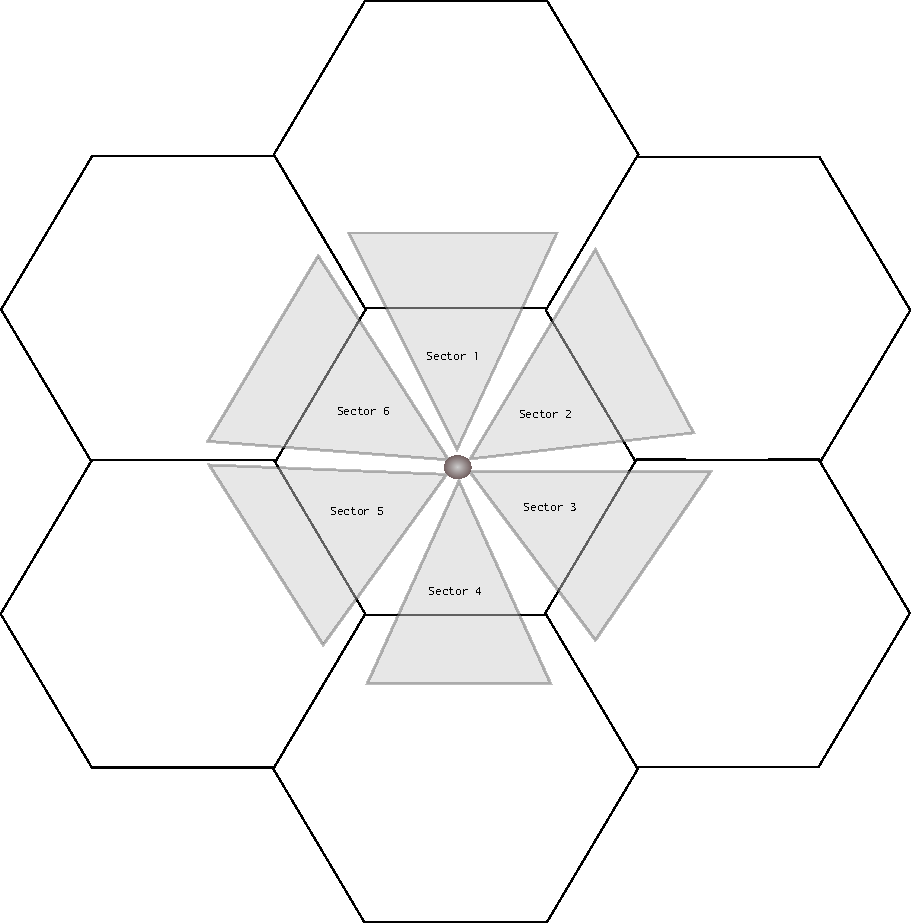
\includegraphics[scale=0.5]{tikz-pics/cellsector.pdf}
	\caption[Cell Sectorization]{Cell sectorisation\cite{GSMSysEngin}.}
	\label{fig:cellsector}
	\end{centering}
\end{figure}

Depending on how many sectors are at a cell, the operating angles of the antennae need to be adjusted accordingly to ensure 360-degree service. If there is only one sector, an omnidirectional antenna is used;, otherwise the antennae operating angles are adjusted to $\frac{360\,^{\circ}}{n}$ where ${n}$ is the number of antennae \cite{Eisenblatter}.

By dividing the cell into sectors the amount of co-channel interference that would occur in a cell is greatly reduced \cite{GSMArchitectureProtocolsServices}. It is important to note that the reduction of co-channel interference is only applicable when the angle of the antenna by which transmission occurs is restricted\cite{GSMArchitectureProtocolsServices}.

Suppose, if a cell using an omnidirectional transceiver is assigned 6 frequencies. If the cell were to be divided into three sectors, where the sectors' antennae are $120^\circ$ apart, the number of interfering co-frequencies shrinks from 6 to 2 and from 6 to one in the case when the cell is divided into 6 sectors \cite{GSMSysEngin,GSM92,GSMArchitectureProtocolsServices}.

Each sector operates one or more elementary transceivers called \gls{TRX}. The number of \gls{TRX} per sector is determined by the expected peak traffic demand that the cell must be able to handle. Each \gls{TRX} can handle 7 to 8 communication links or calls in parallel except the first \gls{TRX}, which handles fewer calls than normal because it is responsible for transmitting cell organisation and protocol information \cite{Eisenblatter}. \glspl{TRX} are able to handle 7-8 calls in parallel due to the use of \gls{FDM} and \gls{TDM} schemes. 

\glspl{TRX} are assigned frequencies, which enable them to provide conversion between digital traffic data on the network side and the radio communication between \glspl{MS}and the \gls{gsm} network\cite{ACOvsEA,FAPOrientationModel}. The frequencies that are used by a cell for communications are discussed in section~\ref{sec:interfacech}.

\subsection{Mobile Switching Centre}

The \gls{MSC} is at the heart of a cellular switching system and forms part of the \gls{NSS}. The \gls{MSC} is responsible for the setting up, routing and supervision of calls between \gls{gsm} subscribers\cite{GSM92,GSMSysEngin}. The \gls{MSC} has interfaces to communicate with \gls{gsm} subscribers (through the \gls{BSS}) on the one hand and with external networks on the other\cite{GSM92}. The \gls{MSC} interfaces with external networks to utilise their superior capability in data transmission as well as for the signalling and communication with other \gls{gsm} network components \cite{GSM92}. 

The most basic functions that an \gls{MSC} is responsible for in a network are the following \cite{wirelesstelcoMullet}:
\begin{itemize}
\item Voice call initialization, routing, control and supervision between subscribers
\item Handover process between two cells
\item Location updating
\item \gls{MS} authentication
\item \gls{SMS} delivery
\item Charging and accounting of services used by subscriber
\item Notification of other network elements
\item Administration input or output processing functions
\end{itemize}

To achieve most of these functions the \gls{MSC} has an integrated \gls{VLR} database that stores call setup information for any \gls{MS} that is currently registered for service with the \gls{MSC} \cite{GSM92,wirelesstelcoMullet}. 

The \glspl{VLR}retrieves this information from the \gls{HLR} that contains all the registered \gls{gsm} subscriber information for the network. This information enables the \gls{MSC} to quickly retrieve the necessary information to set up a call between two clients that want to communicate with each other \cite{GSMSysEngin,GSMSecurInTeleNetwork}.

A requirement for being able to communicate with other network elements such as \gls{PSTN} is the ability to multiplex and demultiplex signals to and from such network elements. This operation is a necessity, since the incoming or outgoing connection bitrate from the source entity might be either too low or too high for the receiving entity.

A typical scenario where this operation proves vital is when a mobile subscriber makes a call to a subscriber on a\gls{PSTN} \@. The connection bit rate needs to be changed at the \gls{MSC} from a wireless connection bitrate to a bitrate suitable for transmission over a\gls{PSTN} \@. In chapter~\ref{chpt:fap} section~\ref{sec:Interference} more information regarding bit rates is presented.

\subsection{Network databases}
The \gls{HLR},  \gls{AUC} and \gls{EIR} are the three `back-end' databases, which store and provide information for the rest of the \gls{gsm} network. In this subsection each one of the databases that form part of the `back-end' is discussed briefly and a description is given of the core functions that each database performs in the network.

\paragraph{Home location register}
--- The \gls{HLR} is a database that permanently stores information pertaining to a given set of subscribers. It needs to store a wide range of subscriber parameters because it is the reference source for anything \gls{gsm} subscriber related in the network\cite{GSMSysEngin}. 

Subscriber parameters that are stored in the database include billing information, routing information, identification numbers, authentication parameters and subscribed services\cite{GSMSysEngin}. The following information is also stored, but the information is of a temporary nature and can change at any time: The current \glspl{VLR}and \gls{MSC} the subscriber is registered with and whether the subscriber is roaming \cite{GSMSysEngin}.

\paragraph{Authentication centre}
--- The AUC is the entity in the \gls{gsm} network that performs security functions and thus stores information that enables it to provide secure over-the-air communication\cite{GSM92,GSMSysEngin}. The information that is stored contains authentication information as well as keys that are used in ciphering information\cite{GSM92,GSMSysEngin}.

During an authentication procedure no ciphering key is ever transmitted over the air; instead a challenge is issued to the mobile that needs to be authenticated. This challenge requires the mobile station to provide the correct \gls{SRES} with regard to the random number generated by the \gls{AUC}\cite{GSM92,GSMSysEngin}. The random number and ciphering keys that are used change with each call that is made; thus an attacker would gain nothing by intercepting a key, since it will change with the next call \cite{GSMSysEngin}.

Each mobile that is registered in the \gls{HLR} database needs to be authenticated and each call that is instantiated needs to retrieve keys from the AUC to establish a secure communication link\cite{GSM92,GSMSysEngin}. The AUC is sometimes included with \gls{HLR} to allow for fast communication between the two databases \cite{GSMSysEngin}.

\paragraph{Equipment identity register}
--- The \gls{EIR} is a database that stores the \gls{IMEI} numbers of all registered mobile equipment that has accessed the network\cite{GSMSysEngin}. Only information about the mobile equipment is stored, nothing about the subscriber or call is stored in the database\cite{GSMSysEngin}.

Typically there is only one \gls{EIR} database per network and interfaces to the \gls{HLR} databases contained in the network\cite{GSMSysEngin}. The \glspl{IMEI} are grouped into three categories: \emph{white list}, \emph{black list} and the \emph{grey list}\cite{GSMSysEngin} The white list contains only the \gls{IMEI} numbers of valid \glspl{MS}; the black list stores the \gls{IMEI} numbers of equipment that has been reported stolen and the grey list stores the \gls{IMEI} numbers of equipment that has some fault (faulty software, wrong make of equipment)\cite{GSMSysEngin}.

\subsection{GSM Network Management Entities}
In a \gls{gsm} network most of the elements that form part of and make the network function are often distributed in a wide geographical area to provide the best network coverage for the customer\cite{GSMSysEngin}. 

For a network to function properly and efficiently network engineers need to be kept up to date on the state of the network and be alerted if \emph{any} problems occur\cite{GSMSysEngin}. For this purpose there are two systems in the \gls{gsm} network architecture that allow for this functionality required by network engineers\cite{GSMSysEngin}. 

One system is called the \gls{OMC}, which is responsible for, centralised regional and local operational and maintenance activities\cite{GSMSysEngin}. The other system is called the \gls{NMC} and unlike the \gls{OMC} it provides global and centralised management for operations and maintenance of the network supported by the OMCs \cite{GSMSysEngin}.

In the following paragraphs more in depth discussions on the critical functions the \gls{OMC} and \gls{NMC} perform is presented.

\paragraph{Operational and Management Centre}
--- The \gls{OMC} is capable of communicating with \gls{gsm} network components using two protocols, namely SS7 and X.25\cite{GSMSysEngin}. The SS7 protocol is usually used when the \gls{OMC} is communicating within the \gls{gsm} network over short and medium distances\cite{GSMSysEngin}. The X.25 protocol is used for large external data transfers\cite{GSMSysEngin}. All communication where the \gls{OMC} is involved occurs over fixed line networks and/or leased lines. The \gls{OMC} is usually used for day-to-day operation of a network \cite{GSMSysEngin}.

The \gls{OMC} has support for alarm handling\cite{GSMSysEngin}. An alarm in a \gls{gsm} network goes off whenever a predefined expected condition does occur. Engineers are able to define the severity of an alarm, which defines who or what is further alerted and if the alarm needs to be escalated to a higher level \cite{GSMSysEngin}.

The \gls{OMC} is also capable of fault management in the \gls{gsm} network\cite{GSMSysEngin}. It is able to activate, deactivate, remove and restore a service manually or automatically on network devices\cite{GSM92}. Various tests can be run and diagnostic information can be retrieved on the network devices to detect any current or future defects \cite{GSMSysEngin}.

\paragraph{Network Management Centre}
--- The \gls{NMC} is similar to the \gls{OMC} but it is not restricted to only regional \gls{gsm} network components as it is in charge of all the \gls{gsm} network components in the network\cite{GSMSysEngin}. The \gls{NMC} provides traffic management for the global network and also monitors high priority alarms such as overloaded or failed \gls{gsm} network components\cite{GSMSysEngin}. It is usually used in long-term planning of a network, but it has the capability to perform certain \gls{OMC} functions when an \gls{OMC} is not staffed. 

\section{GSM Interfaces}
\label{sec:gsminterfaces}
In the \gls{gsm} network all the network components communicate with each other through predefined interfaces. In this section an overview is given of these interfaces between the components.
\begin{description}
  \item{\textbf{Um interface}} --- This interface is the link between an \gls{MS} device and a \gls{BTS} and is also referred to as the \emph{Air} interface since communication occurs wirelessly. The primary protocol used on this interface is the \gls{LAPDm}, which is an extension of the \gls{ISDN} LAPD protocol to accommodate the mobile nature of \gls{MS} devices as well as for the shorter \gls{TDMA} frames which are used in \gls{gsm} networks\cite{wirelesstelcoMullet,GSMSecurInTeleNetwork}.
\item{\textbf{Abis interface}} --- Between the \gls{BTS} and \gls{BSC} the interface used for communication is known as the Abis interface. The only messages that the \gls{BTS} is interested in are those that have to do with management of radio resources\cite{wirelesstelcoMullet,GSMSecurInTeleNetwork}. All other messages are left alone and merely pass through the \gls{BTS} to the \gls{BSC} transparently.
\item{\textbf{A interface}} --- The interface between the \gls{BSC} and \gls{MSC} is known as the A interface. This interface is used for the transfer of information, which is used by the \gls{MSC} to manage BSSs, control connections and manage the mobility of \gls{MS} in its area of service\cite{wirelesstelcoMullet,GSMArchitectureProtocolsServices}.
\item{\textbf{Other Interfaces}} --- The \gls{MSC} has interfaces going from it to databases and other external networks. Each interface connects to a specific database, \gls{MSC} or network and is therefore very specific as to what function it performs\cite{wirelesstelcoMullet,GSMArchitectureProtocolsServices}. An interface going from one \gls{MSC} to another will convey information regarding handling the administration of handover of an \gls{MS} device leaving one administrative area to another MSC's administrative area. The administrative area of an Msc is the section of \gls{BSS} components the Msc is responsible for. The handover procedure is a very delicate process which is described in section~\ref{sec:handover}.
\end{description}

In this section a brief overview was given of the most critical interfaces used by all the network components of the \gls{gsm} network involved. In the next section the difference between a logical channel and a frequency is described. Additionally an outline and overview of all the logical channels defined in the \gls{gsm} is presented. 
\section{GSM channels}
\label{sec:interfacech}
\gls{gsm} defines a series of logical channels, which are used for communication over these interfaces. A distinction needs to be made between channels and frequencies. As discussed earlier, a network is licensed in a certain section of the wireless spectrum for use for commercial communication. This piece of spectrum is referred to as bandwidth and is measured in Hz, therefore $W$ Hz, where $W$ denotes the allocated bandwidth\cite{FundamentalsWirelessCommunication}. This bandwidth W is then divided into N smaller chunks of bandwidth called narrowband chunks. Each N narrowband chunk is a channel and has a width of $W/N$ Hz\cite{FundamentalsWirelessCommunication}. 

Using \gls{TDMA} the \gls{gsm} system is able to provide additional transmission capacity by dividing the frequency into eight equal timeslots \cite{wirelesstelcoMullet}. As can be observed from figure~\ref{fig:GSMfrequencies} each \gls{TDMA} frame has a series of consecutive timeslots. Each timeslot can be used for both uplink and downlink transmission. A \gls{gsm} \emph{channel} is a logical channel and refers to a single timeslot within a \gls{TDMA} frame \cite{wirelesstelcoMullet,GSMArchitectureProtocolsServices}.
\begin{figure}[H]
	\begin{centering}
		\begin{tikzpicture}[]
	\begin{scope}[node distance=0cm]
		\node (startSquare) at (-6.0,0.5) [shape=rectangle,draw=black,minimum height = 0.75cm,minimum width = 0.8cm]{   };
		\node (secondSquare) [right = of startSquare,shape=rectangle,draw=black,minimum height = 0.75cm,minimum width = 0.8cm]{   };
		\node (TS0) [right = of secondSquare, shape=rectangle,draw=black,fill=gray!40,minimum height = 0.75cm,minimum width = 0.8cm]{TS1};
		\node (TS1) [right = of TS0, shape=rectangle,draw=black,fill=gray!40,minimum height = 0.75cm,minimum width = 0.8cm]{TS2};
		\node (TS2) [right = of TS1, shape=rectangle,draw=black,fill=gray!40,minimum height = 0.75cm,minimum width = 0.8cm]{TS3};
		\node (TS3) [right = of TS2, shape=rectangle,draw=black,fill=gray!40,minimum height = 0.75cm,minimum width = 0.8cm]{TS4};
		\node (TS4) [right = of TS3, shape=rectangle,draw=black,fill=gray!40,minimum height = 0.75cm,minimum width = 0.8cm]{TS5};
		\node (TS5) [right = of TS4, shape=rectangle,draw=black,fill=gray!40,minimum height = 0.75cm,minimum width = 0.8cm]{TS6};
		\node (TS6) [right = of TS5, shape=rectangle,draw=black,fill=gray!40,minimum height = 0.75cm,minimum width = 0.8cm]{TS7};
		\node (TS7) [right = of TS6, shape=rectangle,draw=black,fill=gray!40,minimum height = 0.75cm,minimum width = 0.8cm]{TS8};
		\node (secondLastSquare) [right = of TS7, shape=rectangle,draw=black,minimum height = 0.75cm,minimum width = 0.8cm]{   };
		\node (lastSquare) [right = of secondLastSquare, shape=rectangle,draw=black,minimum height = 0.75cm,minimum width = 0.8cm]{   };
	\end{scope}
	\node (startF) at (startSquare.west) [above=1.5cm]{};
	\node (endF) at (lastSquare.east) [above=1.5cm]{};
	\draw [|<->|,thick] (startF) to node [above=0.05cm] {Frequency} (endF);
	\draw[decorate,decoration={brace,amplitude = 0.5cm,raise=0.5cm}] (TS0.west) to node [above=1cm] {TDMA Frame} (TS7.east);
	\node (logicalChannel) [shape=rectangle,draw=black,below = 1.5cm of TS4] {Logical Channel};
	\draw (logicalChannel.north east) to (TS1.south east);
	\draw (logicalChannel.north west) to (TS1.south west);
\end{tikzpicture}

		\caption{TDMA frame and logical channels \cite{wirelesstelcoMullet}}
		\label{fig:GSMfrequencies}
	\end{centering}
\end{figure}
The \gls{gsm} system is therefore able to use the same physical frequency in eight different timeslots without interference as these \emph{logical} channels are used at different times. Therefore using \gls{TDMA} the available frequencies that can be used for communication in \gls{gsm} are increased eightfold \cite{wirelesstelcoMullet}.

Channels are assigned to the uplink and downlink portion of the connection with a duplex separation of 45 MHz in the frequency band to avoid interference between uplink and downlink. There are two types of channels, traffic channels and control channels. \Glspl{TCH} primary purpose is to enable communication of user speech and data and therefore carry no control information \cite{GSMArchitectureProtocolsServices}.

A \gls{TCH} is assigned to an \gls{MS} device when the device indicates that it needs to communicate with another device either with speech or data. When an \gls{MS} has finished with the \gls{TCH} the allocated \gls{TCH} is reclaimed for use by other \gls{MS} devices on the network. This request by the \gls{MS} device occurs using the control frequencies \cite{GSMArchitectureProtocolsServices}.

Control channels are much more actively used in a \gls{gsm} network since they are the primary means by which control and management of the network occurs \cite{GSMArchitectureProtocolsServices}. These channels are used even when the \gls{MS} has no active connection and is in idle mode. This constant activity on the control channels is to keep the network updated with information such as the position of the \gls{MS} (location updating) and signal strength \cite{GSMArchitectureProtocolsServices,GSMSysEngin,Eisenblatter}. 

The control channels are divided into three main channel groups namely \gls{BCH}, \gls{CCCH} and \gls{DCCH} \cite{GSMArchitectureProtocolsServices}. Each of these channel groups contains other channels that aid in the control and management of the network. Each group along with the associated channels will now be briefly discussed.

The first group, \gls{BCH}, consists of three channels:
\begin{description}
  \item{\textbf{\Gls{BCCH}}} --- This channel is broadcast using the very first frequency assigned to a cell. Using this frequency, the channel broadcasts information regarding the network. This information includes radio channel configuration of the current and neighbouring cells, synchronisation information, registration identifiers and most importantly the format of the \gls{CCCH} used by the local \gls{BTS} \cite{GSMArchitectureProtocolsServices}.
  \item{\textbf{\Gls{FCCH}}} --- Synchronisation information is broadcast to the \glspl{MS}to enable them to perform frequency correction on the transmission. Typical synchronisation information on this channel, for instance, is the exact frequency the local \gls{BTS} is using for transmission to enable the \glspl{MS}to attune themselves to the same frequency \cite{GSMArchitectureProtocolsServices}.
  \item{\textbf{\Gls{SCH}}} --- On this channel, identifying information regarding the \gls{BTS} is transmitted. Also on this channel information regarding synchronisation of frames is sent which aids an \gls{MS} to, for example, structure the time frames of \gls{TDMA} frames.
\end{description}

The \gls{FCCH} and \gls{SCH} are always broadcast with the \gls{BCCH} since these channels are needed for the operation of the radio subsystem \cite{GSMArchitectureProtocolsServices}. The \gls{CCCH} is a point-to-point signalling channel that is used to localise an \gls{MS} through the use of paging\cite{GSMArchitectureProtocolsServices}. 

When a \gls{MS} is paged in a \gls{gsm} network, a \gls{CCCH} message is sent to all the cells in the surrounding area of the last known cell the \gls{MS} was recorded to be at\cite{GSMArchitectureProtocolsServices}. The message is sent to surrounding cells in case the \gls{MS} changed location since it was last communication with the network\cite{GSMArchitectureProtocolsServices}. The \gls{MS} receives the paging through the \gls{CCCH} and responds if it is intended for the particular MS\cite{GSMArchitectureProtocolsServices}. The channel is also used to assign dedicated channels \cite{GSMArchitectureProtocolsServices}. The \gls{CCCH} is made up of the following channels:
\begin{description}
  \item{\textbf{\Gls{RACH}}} --- The \gls{RACH} forms the uplink portion of the \gls{CCCH} and is randomly accessed by the \glspl{MS}to request a dedicated channel for a single signalling transaction \cite{GSMArchitectureProtocolsServices}.
  \item{\textbf{\Gls{AGCH}}} --- The \gls{AGCH} forms the downlink part of the \gls{CCCH}\@. It is used by the radio subsystem to assign a \gls{SDCCH} or \gls{TCH} to an \gls{MS} \cite{GSMArchitectureProtocolsServices}.
  \item{\textbf{\Gls{PCH}}} --- The \gls{PCH} also forms part of the downlink portion of the \gls{CCCH}\@. This channel is used by the radio subsystem to page specific \glspl{MS}, which aids in the process of locating an \gls{MS} \cite{GSMArchitectureProtocolsServices}.
\item{\textbf{\Gls{NCH}}} --- This channel is used to inform an \gls{MS} of any incoming group calls or calls that are being broadcast \cite{GSMArchitectureProtocolsServices}.
\end{description}

The last group of signalling channels is referred to as \gls{D/ACCH}. This group of channels has the characteristic that they are a group of bidirectional point-to-point channels \cite{GSMArchitectureProtocolsServices}.
\begin{description}
  \item{\textbf{Stand-alone dedicated control channel (\gls{SDCCH})}} --- This channel is used for communication between the \gls{BSS} and \gls{MS} even when there is no active connection\cite{GSMArchitectureProtocolsServices}. Hence the `stand-alone' since it means that there need not be a \gls{TCH} assigned for communication to occur between the \gls{BSS} and \gls{MS} \cite{GSMArchitectureProtocolsServices}.
  \item{\textbf{\Gls{SACCH}}} --- When a \gls{TCH} or \gls{SDCCH} is assigned, an accompanying \gls{SACCH} is also assigned. The \gls{SACCH} is used to transmit information for optimal radio operation, which can include information on power control of the radio transmitter and synchronisation information\cite{GSMArchitectureProtocolsServices}. Packets must be continuously sent over the \gls{SACCH} as it is used as proof that there is still a physical radio connection \cite{GSMArchitectureProtocolsServices}. When the \gls{MS} has finished using the \gls{SACCH} channel, it transmits a report regard the current results of the radio signal level, which is continuously measured \cite{GSMArchitectureProtocolsServices}.
  \item{\textbf{\Gls{FACCH}}} --- When more bandwidth is required for signalling purposes, the signal of the \gls{TCH} is modified using dynamic pre-emptive multiplexing. The additional bandwidth comes at the expense of the user data transport\cite{GSMArchitectureProtocolsServices}. When a channel is created in this manner it is called a \gls{FACCH} \cite{GSMArchitectureProtocolsServices}.
\end{description}

Finally, one last channel is defined namely the \gls{CBCH}, which shares the same physical channel that the \gls{SDCCH} uses. On this channel messages of the short message service cell broadcast are broadcast\cite{GSMArchitectureProtocolsServices}.

In this section an overview was given of how \emph{logical} channels are used for communication between an \gls{MS}  and \gls{BSS}/\gls{MSC}\@. These three groups of channels collectively enable the \gls{gsm} network to facilitate wireless communication, a very important function for a telecommunication network. The following section dealt with how the network is able to keep a connection to an \gls{MS} alive and allow the \gls{MS} to make calls while the device is moving around geographically within the network.
\section{Handover}
\label{sec:handover}
The handover process in a \gls{gsm} network is initiated when an \gls{MS} with an active call moves outside the coverage area of a cell, \gls{BSS} or \gls{MSC} \cite{GSMArchitectureProtocolsServices,wirelesstelcoMullet,Eisenblatter}. A handover might also be initiated because of measurements indicating bad channel quality\cite{GSMArchitectureProtocolsServices}. 

Various information needs to be migrated across and shared between the components handling the calls to ensure a smooth handover. Not only the \gls{gsm} architecture components that need to continuously share information but also the \gls{MS}\@. The \gls{MS} is required to continuously observe and measure signal strength of up to 6 neighbouring cells. The \gls{MS} does this by monitoring the \gls{BCCH}\cite{GSMArchitectureProtocolsServices,wirelesstelcoMullet}. This information is of course relayed to the \gls{MSC} and \gls{BTS}. The information plays a critical role in the decision process as to which entity will be the best in taking over the administration of the active call\cite{GSMArchitectureProtocolsServices,wirelesstelcoMullet}.

An \gls{MS} can in some cases receive the same \gls{BCCH} from different cells, which are most likely neighbours \cite{GSMArchitectureProtocolsServices}. This problem of duplicate \gls{BCCH} from different cells can be attributed to the frequency reuse in the cellular network as well as to the smaller sector cells forming clusters and therefore overlapping coverage area \cite{GSMArchitectureProtocolsServices}. As discussed in section~\ref{def:cellsector}, cells are divided into sectors, which lessen the problem of co-channel interference. This division into sectors can cause clustering of cells and overlapping of coverage area.

This creates a problem for the \gls{MS} since it needs to distinguish between the two cell measurements as it does not know which measurement belongs to which cell\cite{GSMArchitectureProtocolsServices}. To distinguish between different cells, the \gls{MS} also tries to determine the identity of each cell it is monitoring. Only cells whose identity can be determined reliably are included in the report sent to the BTS\cite{Eisenblatter,GSMArchitectureProtocolsServices,wirelesstelcoMullet}\footnote{When cell identity cannot be determined this can be due to environmental factors like signal strength or to packets getting lost/dropped}. Using this report the handover algorithm is able to decide how to handle the handover, and which cell needs to take over the call\cite{Eisenblatter,GSMArchitectureProtocolsServices,wirelesstelcoMullet}.

Once the cell has been selected, the actual handover process starts. Which has to take into account that the frequency allocated to the incoming call from the other cell does not interfere with other present active calls in the cell receiving the handover\cite{Eisenblatter,GSMArchitectureProtocolsServices,wirelesstelcoMullet}. A frequency interfering with calls currently active in the cell can cause users to hear other conversations from the interfering call, or experience their call being ``dropped'' i.e.\ disconnected\cite{Eisenblatter}. 

There are three core handover procedures when a handover needs to occur in a \gls{gsm} network: \emph{intra-BSC}, \emph{inter-BSC} and \emph{inter-MSC}, each of which involves different \gls{gsm} network components \cite{wirelesstelcoMullet}.

\begin{description}
\item{\textbf{Intra-BSC}} --- Also known as \emph{intercell handover}, this handover is concerned with the transfer of an active call/connection from an \gls{MS} to another cell, which is controlled by the same \gls{BSC} as the current cell\cite{wirelesstelcoMullet,GSMArchitectureProtocolsServices}. The current \gls{BTS} that manages the active call of the \gls{MS} constructs a report containing measurement information from the MS, as well as measurements the \gls{BTS} has taken on signal strength and error bit ratio of the current connection\cite{wirelesstelcoMullet,GSMArchitectureProtocolsServices}. The error bit ratio is defined as how often part of the data being sent over a connection needs to be retransmitted because an error occurred\cite{wirelesstelcoMullet,GSMArchitectureProtocolsServices}. An error can be caused by interference, faulty hardware or the signal strength is fading\cite{wirelesstelcoMullet,GSMArchitectureProtocolsServices}. 

  The constructed report is forwarded to the managing \gls{BSC}. The report is analysed to determine the necessity of handing over the active call to another \gls{BTS}\@. If a handover is deemed necessary, the \gls{BSC} starts by initialising the \gls{BTS} to prepare it to handle the new connection\cite{wirelesstelcoMullet,GSMArchitectureProtocolsServices}.

The \gls{BSC} then notifies the \gls{MS} through the old \gls{BTS} of the new \gls{BTS} identity, and properties of the new connection such as \gls{TCH} frequency, power output etc. After receiving the information about the new connection, the \gls{MS} makes the necessary adjustments for it to continue operating and handling the call on the new connection\cite{wirelesstelcoMullet,GSMArchitectureProtocolsServices}. 

Once all the adjustments have been made the \gls{MS} sends a confirmation to the \gls{BSC} of the successful handover through the new \gls{BTS}\@. The \gls{BSC} instructs the old \gls{BTS} that it must relinquish the use of the \gls{TCH} and its associated \gls{SDCCH} used by the old \gls{MS} call. The \gls{BSC} notifies the \gls{MSC} of the handover as it is used in network operation reports\cite{wirelesstelcoMullet,GSMArchitectureProtocolsServices}.
\item{\textbf{Inter-BSC}} --- In an inter-\gls{BSC} handover a call of an \gls{MS} that is being managed by a \gls{BTS} is transferred to another \gls{BTS}, which has a \emph{different} controlling \gls{BSC}\@. Thus, the call is essentially moved between two \glspl{BSC}, and it is up to the new control \gls{BSC} to select a suitable \gls{BTS} that will actually handle the call of the \gls{MS} being handed over\cite{wirelesstelcoMullet,GSMArchitectureProtocolsServices}.

  This handover occurs because the \gls{MS} is moving or is about to move into a cell that is not controlled by the current \gls{BSC}\@. The current \gls{BSC} detects this and therefore takes the necessary precautions to ensure that the new \gls{BSC} is able to make suitable provision to assume control of the call within one of its BTSs\cite{wirelesstelcoMullet,GSMArchitectureProtocolsServices}.

The \gls{BSC} informs the managing \gls{MSC} that a handover to another \gls{BSC} must occur. The request sent to the \gls{MSC} contains the identity of the cell managed by a different BSC\@. The \gls{MSC} determines the managing \gls{BSC} of the cell in question and notifies it that it must select and prepare the cell for handover. The new \gls{BSC} informs the cell to create a new connection, which will be used by the \gls{MS} once the handover is complete\cite{wirelesstelcoMullet,GSMArchitectureProtocolsServices}.

The new \gls{BSC} informs the \gls{MSC} of the new connection details which the cell will use to handle the handover and maintain the active connection of the \gls{MS}\@\cite{wirelesstelcoMullet}. The \gls{MSC} forwards the connection information to the old \gls{BSC}, which forwards it to the \gls{MS}\@\cite{wirelesstelcoMullet}. The \gls{MS} makes the necessary adjustments for it and then moves on to the new connection. The \gls{MS} informs the new \gls{BSC} that the handover has been completed successfully\cite{wirelesstelcoMullet}. The new \gls{BSC} informs the \gls{MSC}, which then instructs the old \gls{BSC} to relinquish the old connection used by the \gls{MS}\cite{wirelesstelcoMullet,GSMArchitectureProtocolsServices}.
\item{\textbf{Inter-MSC}} --- With an inter-\gls{MSC} handover, control and management of an active call on an \gls{MS} must be transferred to another \gls{BTS}, which resides in a different area that is managed by a different MSC\@\cite{wirelesstelcoMullet}. The handover process follows the same basic formula as the intra-\gls{BSC} and inter-\gls{BSC} handovers once the handover request is made\cite{wirelesstelcoMullet,GSMArchitectureProtocolsServices}.
The \gls{BSC} managing the \gls{BTS} to which the \gls{MS} is going to be handed over is to be determined by the MSC\@\cite{wirelesstelcoMullet}. The \gls{BSC} is notified by the new managing \gls{MSC} that certain \glspl{BTS} must bring a new connection online for the incoming \gls{MS}; the network components upstream\footnote{components upstream are the network components which are higher up in the managing structure. In this instance, \gls{BTS} -- \gls{BSC} -- \gls{MSC}\@.} are notified\cite{wirelesstelcoMullet,GSMArchitectureProtocolsServices}.

The new \gls{MSC} informs the old \gls{MSC} of the new connection details. The old \gls{MSC} transfers the connection information to the \gls{MS} that is going to be a handed over to another \gls{BTS}\@\cite{wirelesstelcoMullet}. The \gls{MS} makes the corresponding adjustments and then starts operating on the new connection. The \gls{MS} informs the \gls{BSC} of the successful handover\cite{wirelesstelcoMullet,GSMArchitectureProtocolsServices}. 

  The \gls{BSC} in turn informs the new \gls{MSC}, which in turn informs the old \gls{MSC} that the handover was successful. The \gls{MSC} then instructs the \gls{BSC} to ensure that the old connection resources are relinquished by the \gls{BTS}.
\end{description}

In this section a discussion was presented on the handover process in \gls{gsm} network. The effect this has on the channel selected as well as the different handover procedures was highlighted. 
\section{Summary}
In this chapter a broad discussion was given of modern cellular technology, specifically \gls{gsm} cellular network technology. A brief history on how \gls{gsm} was developed to be the most widely used cellular technology in use today was provided. The \gls{gsm} architecture components followed. In the \gls{gsm} architecture all the network components present in a modern \gls{gsm} network were identified.

Following the discussion of the \gls{gsm} network components, a broad overview was given of the communication interfaces used between the \gls{gsm} network components to communicate with each other. This was followed by a definition of the \gls{gsm} channels, which are used on the interfaces to communicate information.

The chapter concluded with the handover process, which is used to allow an \gls{MS} device to move freely geographically within the network. 
